\apendice{Plan de Proyecto Software}

\section{Introducción}
La metodología de trabajo seguida ha sido la metodología Kanban \cite{wiki:Kanban}. El método Kanban toma la filosofía de las metodologías evolutivas e incrementales haciendo énfasis en la intención de la entrega del producto justo a tiempo.

Uno de los elementos clave de esta metodología es el tablero Kanban \cite{TableroKanban}. Este tablero está dividido en una serie de apartados definidos que representarán el flujo de trabajo de las tareas a realizar. A este tablero se van añadiendo las tareas que se van a realizar, y estas van viajando de una fase de desarrollo de la tarea a otra. Habrá una fase de desarrollo final que represente que esa tarea esta completada que será la última fase a la que accedan todas las tareas.

Las tareas del tablero Kanban pueden ser clasificadas en distintas etiquetas según el ámbito de la tarea.

Un videojuego es un producto software cuyo grado de completitud es difícil de estimar, un bug puede retrasar mucho la ejecución. Es además frecuente que no se coumplan los plazos de desarrollo de los videojuegos. Los tableros Kanban puede resultar útil para enfrentar estos problemas ya que son útiles para:
\begin{itemize}
\item
Ayudar a visualizar el flujo de trabajo, facilitando identificar adelantos y retrasos y conocer el estado del proyecto.
\item
Identificar y reducir cuellos de botella.
\item
Es adecuado para desarrollos incrementales, especialmente aquellos que hagan uso de integración y despliegue continuos.
\end{itemize}

\section{Planificación temporal}
\subsection{Tablero Kanban}
El tablero Kanban diseñado para este proyecto es uno en el que las tareas pueden estar en cuatro posibles fases de desarrollo:
\begin{itemize}
\item
\textbf{To do:} En esta fase se almacenan las tareas que han sido identificadas y se tiene planeado llevar a cabo pero cuyo desarrollo no ha comenzado todavía.
\item
\textbf{In progress:} La tarea está siendo llevada a cabo.
\item
\textbf{QA/Testing:} Fase de revisión de la tarea. Se comprueba que se ha realizado correctamente.
\item
\textbf{Done} Esta es la fase final del tablero. Todas las tareas que llegan a esta fase se dan por terminadas.
\end{itemize} 

El tablero Kanban se puede encontrar en el repositorio de Github del proyecto en el apartado de ''Projects'' (\url{https://github.com/Kencho/mri1001-tfg/projects/1})

\begin{figure}[h]
\centering
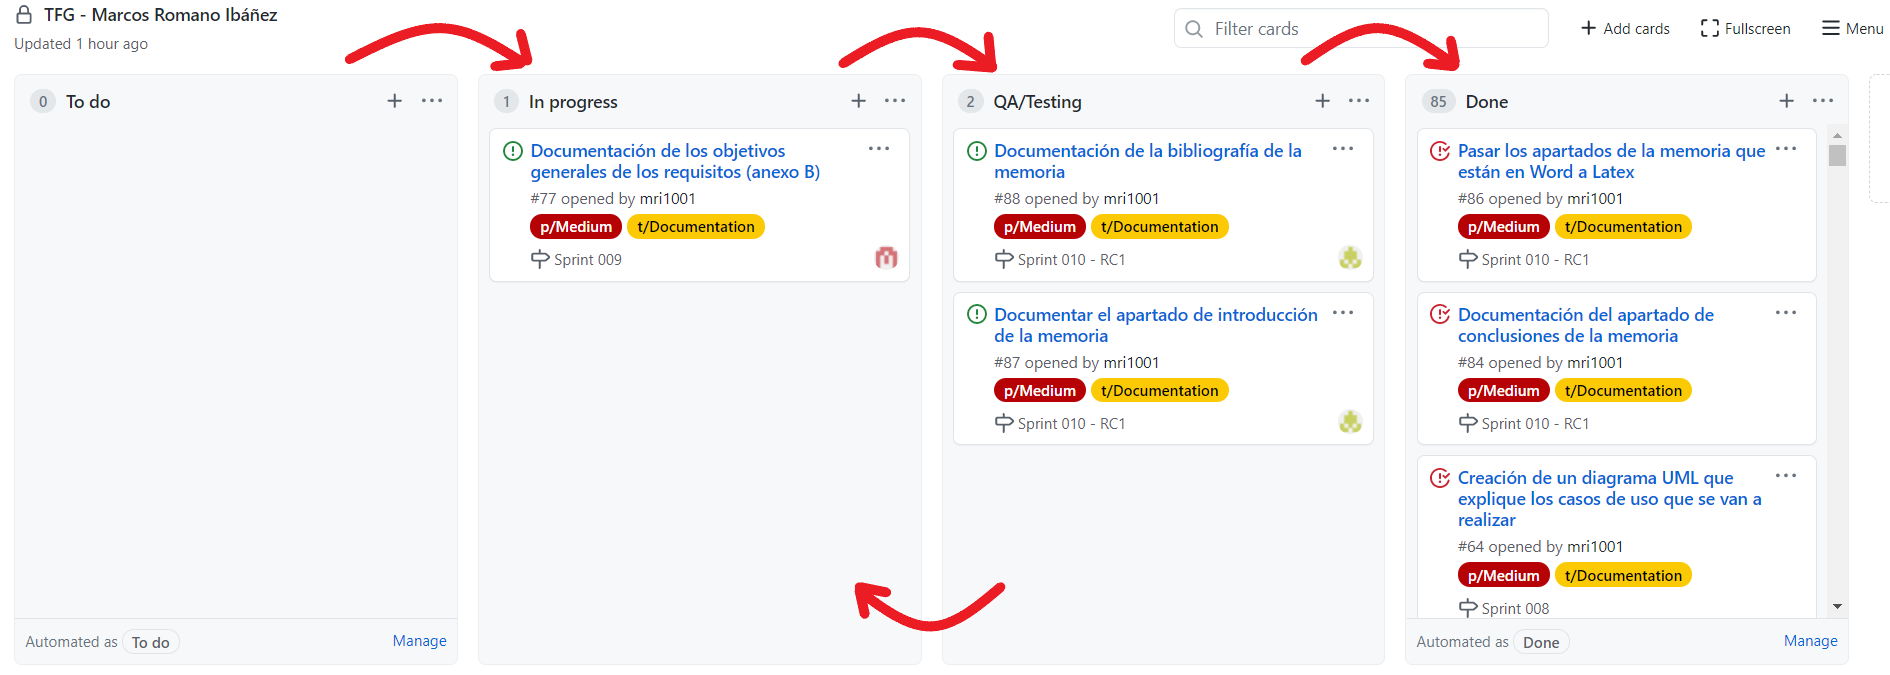
\includegraphics[scale=0.3]{Anexos/Anexo_A/Tablero_Kanban}
\caption{Captura de pantalla del tablero Kanban utilizado}
\end{figure}
\clearpage

\subsection{Fases del desarrollo}
El proyecto consta de tres fases separadas del desarrollo:
\begin{itemize}
\item
La fase de desarrollo del proyecto en la que se implementan las mecánicas y los elementos del juego. Esta fase es la que más tiempo lleva, durando desde el 1 de febrero de 2021 hasta el 16 de mayo de 2021. Al final del desarrollo de esta fase, salvo por algunos errores que quedaron pendientes de solucionar, los objetivos planteados para esta fase se cumplieron satisfactoriamente.
\item
La fase de beta en la que se considera que el juego ya ha tomado forma como producto software y se entra a una fase centrada en la resolución de errores y documentación de la memoria. Esta fase dura desde el 17 de mayo de 2021 hasta el 6 de junio de 2021.\\
Durante el desarrollo de esta fase se realizaron refactorizaciones (facilitan encontrar errores y realizar cambios), corrigieron errores, se documentó la memoria y se añadieron recursos estéticos para mejorar la sensación de juego (principalmente sonidos).\\
Se invirtió demasiado tiempo en la implementación de los recursos que mejorasen la sensación de juego (sobre todo la opción de modificación del volumen de la música) dedicándose poco tiempo a la memoria y ralentizando el cierre del proyecto.
\item
La fase de ''Release candidate'' que dura una semana donde se comprueba que el desarrollo está listo, el código es accesible y el proyecto se puede descargar y ejecutar satisfactoriamente. A la hora de llevar a cabo esta fase requirió más trabajo del esperado ya que el retraso generado en la fase de beta obligó a arrastrar algunas de las tareas de esta a la ''Release candidate''. Sin embargo este retraso es fue asumible debido a que se hizo la planificación temporal contando con un colchón de tiempo por si algún contratiempo retrasaba el proyecto.
\end{itemize}

\subsection{Cuellos de botellas}
Durante el desarrollo del proyecto se han encontrado tres cuellos de botellas en los que la realización de ciertas tareas ha llevado más tiempo del esperado:
\begin{itemize}
\item
La implementación del Player: La implementación del Player y todas las mecánicas relativas a este se tenía la percepción de que en 25-30 horas estarían implementadas. Sin embargo este proceso se alargó hasta las 48 horas.
\item
La implementación del sistema de colisiones estaba planeada para durar una semana de trabajo. Sin embargo se alargó hasta las dos.
\item
No estaba planeado añadir la opción de modificación del volumen de la música. Añadir esta tarea improvisada sobre la marcha, requirió de dos días que estaba planeado se dedicasen a tareas ya planificadas.
\end{itemize} 

\section{Estudio de viabilidad}
A continuación se va a proceder a realizar el estudio de viabilidad del proyecto. Dejar claro que este estudio de viabilidad no va a ser representativo de un estudio de viabilidad de un videojuego, ya que este TFG se ha centrado sobre todo en el punto de vista del programador obviando el resto de vertientes del proyecto como el apartado artístico o sonoro en los cuales se ha hecho uso de recursos de la comunidad gratuitos, de manera que los sueldos y otros gastos asociados a estos trabajadores no van a constar en el estudio de viabilidad económica.

Otro tema que diferirá de otros videojuegos desarrollados con Unity será que si en el último ejercicio fiscal los ingresos fueron superiores a 100.000 dolares estadounidenses, se está obligado a comprar la edición profesional de Unity \cite{FAQUnity}. Al no comercializar el juego no es necesario estar pendiente de estos gastos. Presuponiendo también que es el primer producto desarrollado con Unity no habrá precedentes que obliguen a obtener la licencia profesional de Unity.

\subsection{Viabilidad económica}
Se va a valorar la viabilidad del proyecto desde el punto de vista económico. Para ello se evaluarán dos aspectos: los costes y los beneficios.\\
Los cálculos se harán asumiendo que el proyecto lo lleve a cabo una empresa y que se tenga liquidez suficiente como para no requerir financiamiento.

\subsubsection{Costes}
\textbf{Costes de recursos humanos:}
El salario medio de un programador de videojuegos en España es de 32.100 € \cite{Sueldo}. Sin embargo el sueldo varía mucho de un programador senior a uno junior. Se va a asumir que en este caso el programador es junior (es un alumno de 4º). El sueldo neto medio mensual de un programador junior es de 1.160 €.

\begin{figure}[h]
\centering
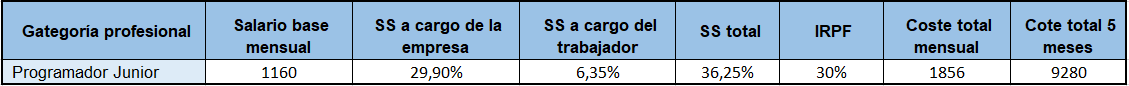
\includegraphics[scale=0.6]{Anexos/Anexo_A/Sueldo_trabajador}
\caption{Tabla de Excel con el sueldo calculado del trabajador}
\end{figure}

\textbf{Activos:}
El único activo que ha sido necesario para el desarrollo del proyecto ha sido el ordenador portátil en el que se ha creado el videojuego. Se estima que la vida útil de este activo será de 5 años, con lo que se amortizará en ese tiempo. En los 5 meses que ha durado el proyecto el coste de amortización del portátil es de 100 €

Las ventas no superarán los 100.000 €, así no hará falta pagar la versión profesional de Unity, resultando el software utilizado gratuito.

\begin{figure}[h]
\centering
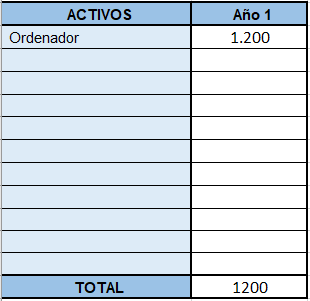
\includegraphics[scale=1]{Anexos/Anexo_A/Activos}
\caption{Tabla de Excel con los activos del proyecto}
\end{figure}

\subsubsection{Beneficios}
La media de unidades vendidas de por los videojuegos indies (desarrollados por muy pocas personas) está en torno a las 1.500 € unidades \cite{Unidades}. Si se desea vender el juego, el precio máximo que podría alcanzar es de 2€ por copia vendida, generando 3.000 € de ingresos.

\subsubsection{Balance}
El proyecto actualmente no es viable económicamente. Sin embargo cabe destacar que el principal motivo de esto es el precio del juego (2 euros). Es un precio bajo, pero actualmente tiene muy poco contenido el juego y no tiene sentido pedir más dinero por él.\\
Dejar claro también que con un 2 meses de producción (centrados en generar contenido jugable) más el juego se podría cobrar dignamente a 5 € y con otros 4 meses a 10 € o incluso 15 €.

\textbf{Balance actual:}
\begin{figure}[h]
\centering
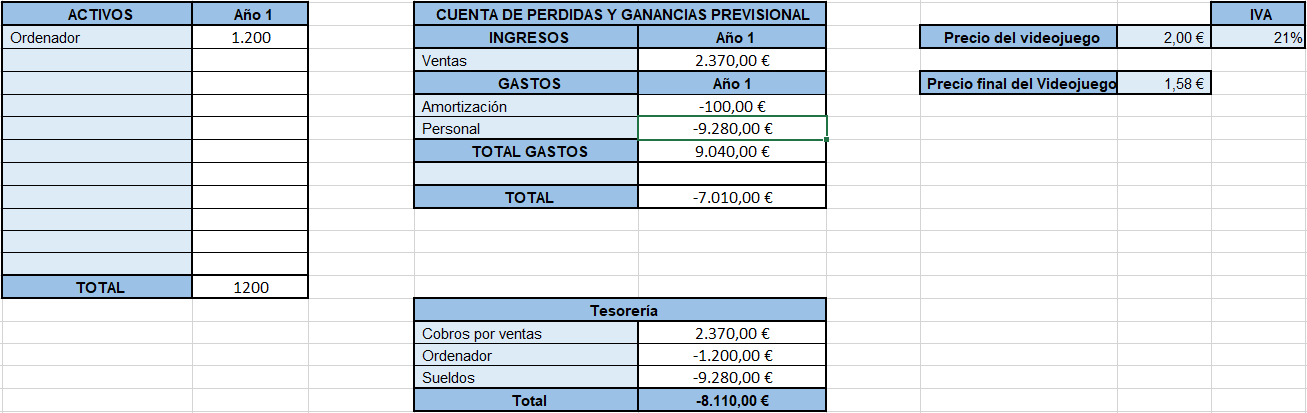
\includegraphics[scale=0.45]{Anexos/Anexo_A/Balance_actual}
\caption{Tabla de Excel con el balance del proyecto}
\end{figure}

\textbf{Balance a los 2 meses:}
\begin{figure}[h]
\centering
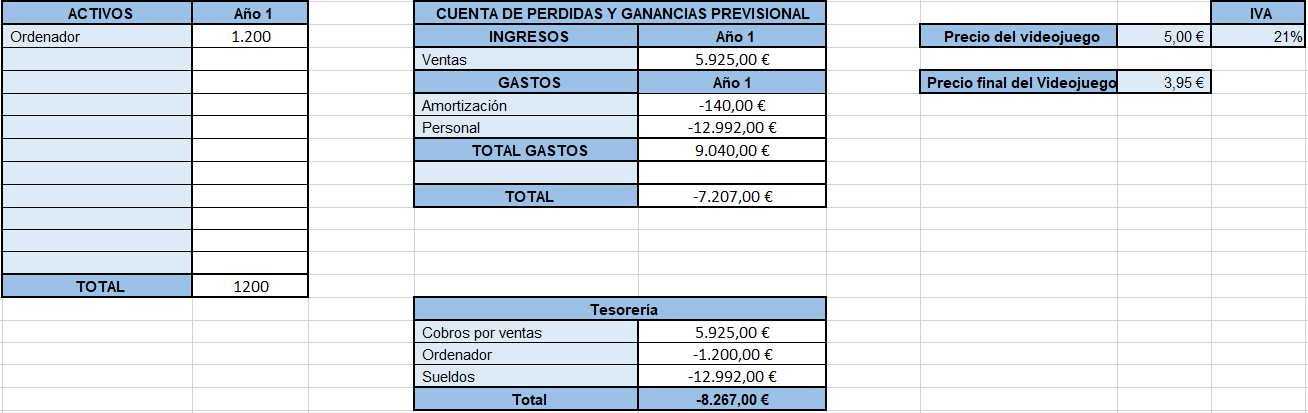
\includegraphics[scale=0.45]{Anexos/Anexo_A/Balance_2meses}
\caption{Tabla de Excel con el balance del proyecto con 2 meses más de desarrollo}
\end{figure}

\textbf{Balance a los 4 meses}
A los 4 meses de trabajo hay dos opciones:

Que el producto terminado posea el contenido suficiente pero su calidad deje algo que desear, en cuyo caso el juego se cobrará a 10 €.

\clearpage
\begin{figure}[h]
\centering
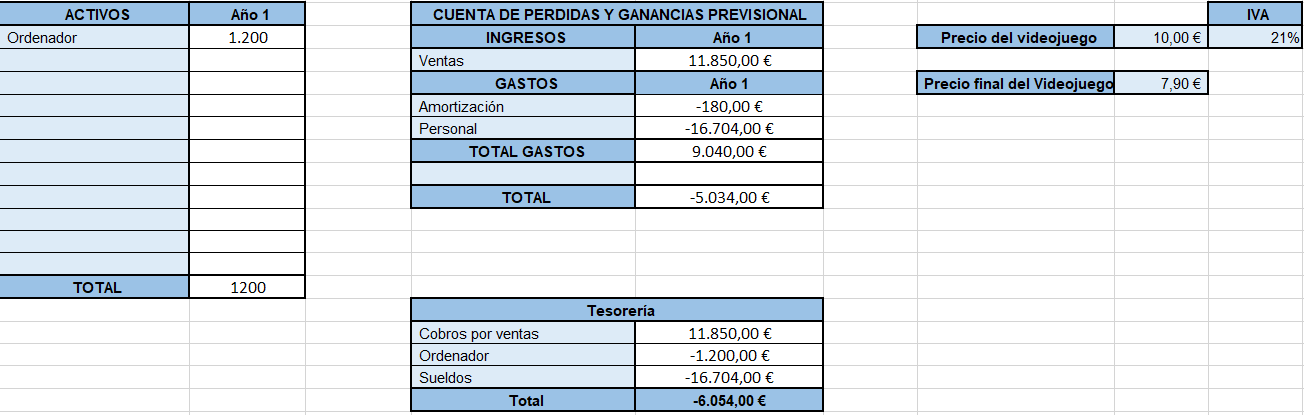
\includegraphics[scale=0.45]{Anexos/Anexo_A/Balance_4meses}
\caption{Tabla de Excel con el balance del proyecto con 4 meses más de desarrollo (precio del videojuego 10 €)}
\end{figure}

Que el producto terminado posea el contenido suficiente y haya sobrado tiempo para mejorar el apartado artístico. La calidad del juego es buena y se puede pedir 15 € por él.
\begin{figure}[h]
\centering
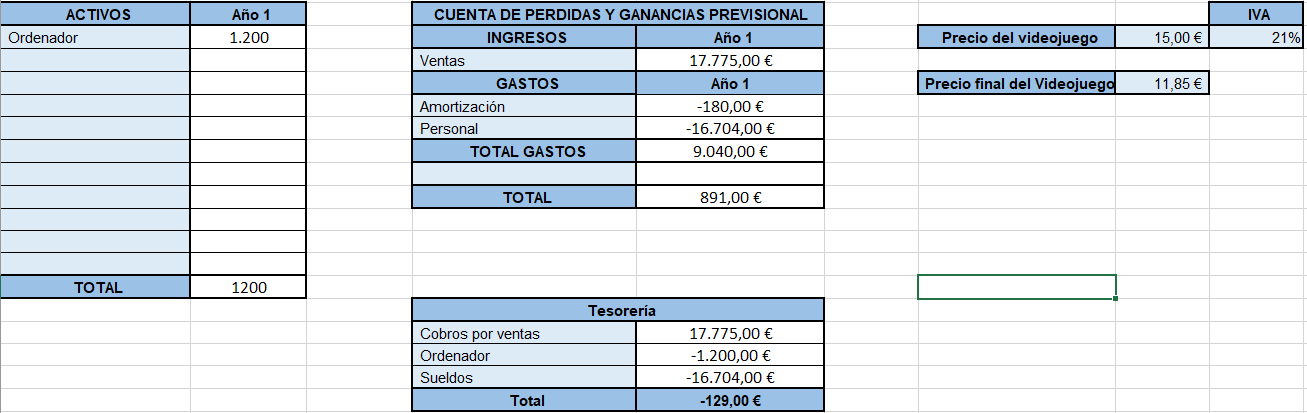
\includegraphics[scale=0.45]{Anexos/Anexo_A/Balance_4meses_optimista}
\caption{Tabla de Excel con el balance del proyecto con 4 meses más de desarrollo (precio del videojuego 15 €)}
\end{figure}

\subsection{Viabilidad legal}
En cuanto a la viabilidad legal, afortunadamente para este proyecto es sencillo el marco legal.

Los derechos de autoría corresponderán al desarrollador del videojuego y los de explotación a también a él. En caso de trabajar para una empresa los derechos de explotación se transmitirán a esta \cite{PropiedadIntelectual}.

Los elementos artísticos utilizados en el videojuego han sido obtenidos de personas que los han cedido para su libre uso. Todo este contenido se han regido por distintas licencias de CopyRigth, pero todas las estas licencias permiten su libre uso, pero requiriendo mencionar al autor.

\clearpage
Esas licencias son:
\begin{itemize}
\item
Attribution 4.0 International (\url{https://creativecommons.org/licenses/by/4.0/})
\item
Attribution 3.0 Unported (\url{https://creativecommons.org/licenses/by/3.0/})
\item
Attribution 2.0 Generic (\url{https://creativecommons.org/licenses/by/2.0/})
\item
Attribution 1.0 Generic (\url{https://creativecommons.org/licenses/by/1.0/})
\end{itemize}